% haven't finished, just draft
\section{Experimental Results}
\label{sec:eval}
%
%\begin{itemize}
%\item Experiment set up - data sources, computing resources, etc.
%\item Comparison of the stats of the original free association norm graph
%and our expanded mind drifting graph. Show fragments of the graph,
%give online demo URL.
%\item Prediction of free association - using another FA data set.
%\item Accuracy of term similarity - compare the results of LSA, ESA, FA norm
%and MD on the following data sets: WS-89, WS-271, WS-353
%\cite{FinkelsteinGMRSWR02}.
%\item Accuracy of short text similarity -  compare the results of LSA, ESA
%and MD on STSS-65 and STSS-131.
%\item Scalability results.
%\item Execution time - compare LSA, ESA and MD on WS-353
%\end{itemize}
%


This section primarily evaluates two association networks, one
constructed only using the original free association norms (denoted
as $AN_{free}$), and the other constructed through the approach
proposed in \secref{sec:approach} (denoted as $AN_{wiki}$). The
results on $AN_{free}$ show the usefulness as well as limitations of free association
norms, while the results
on $AN_{wiki}$ validate the added benefits of Wikipedia structures 
in working around the two limitations of $AN_{free}$, leading to
better performance in semantic relatedness computation tasks.~\footnote{A demo of our system is available at
\url{http://adapt.seiee.sjtu.edu.cn/~keyang/assoc/}.}
%We first show the original free association network's usefulness
%and limitation in computing semantic relatedness in \secref{sec:free}.
%We then show the proposed $AN_{wiki}$'s ability to predicate a real
%free association network in \secref{sec:predict}. Next, in
%\secref{sec:term} and \secref{sec:text}, our association network,
%which combines cognitive signals from free association norms and co-occurrence
%signals from Wikipedia, shows state-of-the-art results in computing
%term-to-term relatedness as well as short text relatedness.
%We then show how the four new types of co-occurrence in Wikipedia
%complement the commonly used sentence-level co-occurrences, and how
%the signals from free association norms further improve the overall result,
%in \secref{sec:comparison1}. The next experiment demonstrates
%the two term relatedness algorithms, $cos_{same}$ and $cos_{cross}$,
%capture not only different, but also complementary signals
%in \secref{sec:comparison2}. Finally, in \secref{sec:time}, we record
%the execution time of the two main tasks, compared with ESAlib\cite{},
%a widely used implementation of ESA.

%Next we compare $AN_{wiki}$ with a bunch of state-of-the-art models the
%results of term relatedness measuring and short text relatedness measuring in \secref{sec:term} and \secref{sec:text} respectively.
%first describes the data sources used to build and some statistics about the two association networks evaluated in the experiments, one constructed only using the free association norms (denoted as $AN_{free}$), and the other constructed through the approach proposed in \secref{sec:statistics} (denoted as $AN_{wiki}$). We then motivate our work of constructing such a large-scale, comprehensive association network by showing the free association network's usefulness and limitation in semantic relatedness measuring in \secref{sec:free}. Next, we show $AN_{wiki}$'s ability of predicting association on another free association dataset\cite{} in \secref{sec:predict}. Next we present and compare with a bunch of state-of-the-art models the results of term relatedness measuring and short text relatedness measuring in \secref{sec:term} and \secref{sec:text} respectively. Next, we show the four types of co-occurrence we add to complement slc as well as the free association data's contribution to our overall result on the two tasks by adding one at a time in \secref{sec:comparison1}. Next, we show in our term relatedness measuring algorithm, $cos_{same}$ and $cos_{cross}$ capture not only different, but also complementary signals in \secref{sec:comparison2}. Finally, in \secref{sec:time} we test our execution time on the two tasks, compared with ESAlib\cite{}, a widely used implementation of ESA.
%
\subsection{Data sources and statistics}
\label{sec:statistics}

The original Florida free association norms data
contains 5,019 cue words (which form the set of {\em normed words})
and a total of 72,176 cue-response pairs.
63,619 of these pairs contain responses that are also normed words.
These pairs are called {\em normed pairs} 
with known forward (cue-to-target) and backward (from target-to-cue) strengths.

%These pairs (referred as {\em normed pairs}) are particularly important
%for researchers wishing to select pairs with known forward (cue-to-target)
%and backward (from target-to-cue) strengths. \cite{Nelson:2004},
%which is indeed the case in our semantic relatedness measuring algorithm.

Our baseline association network, $AN_{free}$, is made up of the 5019
normed words as vertices and the 63,619 normed pairs as directed edges.
Each edge carries a normalized weight $w(u, v)$, which is
proportional to $Pr(v ~|~ u)$,
%and as only the normed pairs are used, normalization needs to be conducted to meet the constraint specified in \eqref{eq:normalize} .
Note, in $AN_{free}$, each word forms a super node by itself, as we aim to
evaluate usefulness of the original free association norms, without
depending on additional knowledge (e.g., Wikipedia) to construct super nodes.

Our proposed synthetic association network, $AN_{wiki}$, consists of 17,469
vertices (super nodes) and 107M directed edges.
% The minimum fanout is 91, and the maximum fanout is 17,382.
This network is constructed using the 20,000 most
common English words (with stop words removed) as given $T_0$, and using
a Wikipedia dump from July, 2014.
% , which consists of 4.6M pages and 1M categories.

Our test set for evaluting term relatedness is the well-known
{\em WordSimilarity-353} \cite{WS353} (a.k.a. WS-353 with 353 word pairs), 
%WS-353\cite{WS353} consists of 353 pairs of words annotated by 13
%human subjects, on a scale of 0 (unrelated) to 10 (very closely
%related or identical). RG-65\cite{RG65} consists of 65 word pairs
%ranging from synonymy pairs (e.g., car - automobile) to completely
%unrelated terms (e.g., noon - string). These pairs were annotated by
%51 human subjects. All the nouns pairs are non-technical words
%scored on a scale of 0 (not-related) to 4 (perfect synonymy).
%MC-30\cite{MC30} contains 30 word pairs, which are a subset of both
%WS-353 and RG-65, rated by 38 human subjects, on a scale of 0 to 4.
%MC-30 is a subset in the WS-353 that contains 30 simple,
%generic English words.
%Unlike the Miller-Charles data set, which consists only of
%single generic words, the
%WS-353 set, on the other hand, includes phrases (e.g., “Wednesday news”),
%proper nouns and technical terms, therefore posing an additional degree of difficulty for any relatedness metric.
%

For testing short text similarity, we use the well-known public set
{\em Li30} \cite{li06}, comprising 30 pairs of short texts. A newly constructed dataset
STSS-131 \cite{STSS131} is used to tune the parameter $K$ decribed in
Algorithm \ref{algo:expand}.


\subsection{$AN_{free}$ v.s. $AN_{wiki}$}
\label{sec:free}
To illustrate the usefulness of free association network, as well as
its limitation in semantic relatedness computation, we create WS-227,
a subset of WS-353, in which all words belong to some vertex in
$AN_{free}$.

The baseline algorithm with \eqref{eq:baseline} as its metric 
is denoted by $AN^0$, while the revised algorithm with \eqref{eq:revised} as its metric is denoted by $AN^+$.
We apply $AN^0$ and $AN^+$
using $AN_{free}$ and $AN_{wiki}$ on WS-227 and WS-353, and compare the performance measured in Spearman
correlation with two other well-known algorithms, namely
LSA \cite{LSA} and ESA \cite{ESA}, in \tabref{tab:ws227}. The result
for LSA is obtained from the widely used online
portal\footnote{http://lsa.colorado.edu/}, while the result for ESA is obtained from
ESAlib\footnote{http://ticcky.github.io/esalib/}.
%Note that both implementations reach quite similar correlation in WS-353 compared with the results reported in the original papers. The result for $AN_{wiki}$ is also included here for comparison.

We observe the following:
1) $AN_{free}^+$ performs better than LSA and ESA on WS-227,
despite its relatively small size, which suggests that free
association can be useful in computing semantic relatedness.
2) However, when tested on WS-353, due to its limited vocabulary,
$AN_{free}^+$ shows a drastic degrade in performance, which reflects
one of its primary limitations. Conversely, $AN_{wiki}$, of a larger lexical
coverage, performs consistently well on both WS-227 and WS-353.
3) Due to $AN_{free}$'s another limitation, sparseness, $AN_{free}^0$ 
exhibits sub-optimal performance on both WS-227 and WS-353; while 
$AN_{free}^+$ shows a significant improvement as the sparseness 
problem is alleviated by leveraging the latent bridge vertices. 
4) Though the best performance is obtained by $AN_{wiki}^+$, its advantage
over $AN_{wiki}^0$ is not large. We argue that it is because by 
reverse-engineering the association strength into an aggregation 
function of a vector of structured co-occurrence,
$AN_{wiki}$ alleviates sparseness by enabling to infer the edge weights missing 
in $AN_{free}$. 

\begin{table}[ht]
\centering
\caption{Spearman correlation on two WS datasets}
\begin{tabular}{lccc}
\hline
Methods & WS-227 & WS-353 \\
\hline
LSA & 0.542 & 0.579 \\
ESA & 0.727 & 0.744 \\
$AN_{free}^0$ & 0.645 & 0.476 \\
$AN_{free}^+$ & 0.752 & 0.512 \\
$AN_{wiki}^0$ & 0.758 & 0.785 \\
$AN_{wiki}^+$ & {\bf0.782} & {\bf0.813} \\
\hline
\end{tabular}
\label{tab:ws227}
\end{table}

\subsection{Prediction of free association}
\label{sec:predict}

In this experiment, we evaluate if $AN_{wiki}$ can be used to
predict free association strengths given by humans. We compute
Spearman correlation between scores predicted by a number of
competing methods \cite{asso09} and the human association strength
computed from the Kent's free association norms \shortcite{kent1910study}.
Our method is just mapping the two terms to vertex $u$ and $v$, and
assigning $w(u,v)$ as predicted association strength. 
%\KZ{Need to explain a bit more what each of these methods are. And how
%we compute the association strength - do we just give the weight on the
%edges directly?}
%\cite{}, for evaluating agreement between predicted associations and human
%associations, and compare with a bunch of popular metrics.

% The ``global" column
% shows correlations between the rankings among all pairs of words in
% the dataset; while the ``local" column gives the average correlation
% scores over pairs of words grouped by cue words. 

As is shown in \tabref{tab:predict},
$AN_{wiki}$ does a reasonable job in simulating free association,
compared with other common approaches. And as a reference, the
Spearman correlation between the human labeled scores of Kent dataset and those of the Minnesota
dataset \cite{Minnesota} using the same set of cue words is 0.4,
which can be viewed as an upper bound for computer-based systems.
\begin{table}[ht]
\centering
\caption{Association Prediction}
\begin{tabular}{lcc}
\hline
Methods & Spearman  \\
\hline
Cond. Prob. & 0.31 \\
SCI & 0.34 \\
PMI & 0.28 \\
Dice/Jaccard & 0.32 \\
$AN_{wiki}$ & {\bf0.37} \\
% Methods & global & local (per cue word) \\
% \hline
% Cond. Prob. & 0.31 & 0.35 \\
% SCI & 0.34 & 0.41 \\
% PMI & 0.28 & 0.34 \\
% Dice/Jaccard & 0.32 & 0.4 \\
% $AN_{wiki}$ & {\bf0.37} & {\bf0.41} \\
\hline
\end{tabular}
\label{tab:predict}
\end{table}


\subsection{End-to-end tasks: term \& short text relatedness}
\label{sec:term}

\tabref{tab:ws353} compares $AN_{wiki}$ with a number of previous
approaches on the term relatedness computation using WS-353 dataset. 
Our association network achieves
state-of-the-art results on correlation with human scores.
%Recall that, when constructing $u_{to}$ and $u_{from}$, we use only
%the top $L$ weighted dimensions  to remove noises. 

\begin{table}[ht]
\centering
\caption{Spearman correlation on WS-353 dataset}
\begin{tabular}{lccc}
\hline
Methods & Spearman \\
\hline
Resnik \shortcite{Resnik:1995}  & 0.353 \\
LSA-Landauer \shortcite{LSA_353}  & 0.581 \\
Lin \shortcite{Lin:1998} & 0.348 \\
Roget-Jarmasz \shortcite{Roget_Jarmasz} & 0.415 \\
ESA-Gabrilovich \shortcite{ESA}  & 0.75 \\
Agirre \shortcite{Agirre:2009} & 0.78 \\
Reisinger \shortcite{reisinger2010multi} & 0.77 \\
SSA-Hassan \shortcite{SSA} & 0.629 \\
TSA-Radinsky \shortcite{TSA}  & 0.80 \\
CLEAR-Halawi \shortcite{CLEAR}  & 0.810 \\
Xu \shortcite{NET}  & 0.683 \\
$AN_{wiki}$  & {\bf0.813} \\
\hline
\end{tabular}
\label{tab:ws353}
\end{table}

%\subsection{Short text relatedness}
%\label{sec:text}
\tabref{tab:li30} shows that our association network outperforms all
existing approaches by significant margins on short text similarity
task.

Recall that, Algorithm \ref{algo:expand} is parameterized by $K$
determining the extent of expansion. Our reported results use
$K=10$, empirically tuned based on STSS-131 dataset.

\begin{table}[ht]
\centering
\caption{Pearson and Spearman correlation on Li30 dataset}
\begin{tabular}{lcc}
\hline
Methods& Pearson & Spearman \\
\hline
STASIS-Li \shortcite{li06} & 0.816 & 0.813 \\
LIU \shortcite{Liu_STSS} & 0.841 & 0.854 \\
%FENG \shortcite{Feng_STSS} & 0.756 & 0.608 \\
LSA-OShea \shortcite{LSA_STSS} & 0.838 & 0.871 \\
STS-Islam \shortcite{STS} & 0.853 & 0.838 \\
Omiotis-Tsatsaronis \shortcite{Omiotis} & 0.856 & 0.891 \\
WSD-STS-Ho \shortcite{SPD-STS} & 0.864 & 0.834 \\
SPD-STS-Ho \shortcite{SPD-STS} & 0.895 & 0.903 \\
SSA-Hassan \shortcite{SSA} & 0.881 & 0.878 \\
LDA-Guo \shortcite{WTMF} & 0.842 & 0.866 \\
WTMF-Guo \shortcite{WTMF} & 0.898 & 0.909 \\
WTMF+PK-Guo \shortcite{WTMF+PK} & 0.902 & -- \\
$AN_{wiki}$ & {\bf0.942} & {\bf0.940} \\
\hline
\end{tabular}
\label{tab:li30}
\end{table}

\subsection{Effects of different co-occurrences and free association training}
\label{sec:comparison1}
In this experiment, we compare an association network built from
only sentence-level co-occurrences (slc), an association network with 5 types of
co-occurrences uniformly combined (uniform), and our proposed network, which
comes with weights trained from free association norms.
%
%We use slc alone to build the association network $AN_{wiki}$(slc), and set the 5 weight parameters combining different types of co-occurrence by uniform distribution, i.e., all of the 5 parameters are set to 1/5, to build the association network $AN_{wiki}$(uniform). $AN_{wiki}$(train) is just the association network used in above experiments, in which the weight parameters are trained using free association norms.
%
%We compare the three association networks on our two end-to-end applications,
%and the results is shown in
\tabref{tab:comparison1} gives rise to these observations:
i) $AN_{wiki}$(uniform) outperforms $AN_{wiki}$(slc) by a large margin
on both tasks, which shows that the four additional types of co-occurrences
are useful in capturing signals not available in slc;
ii) $AN_{wiki}$ further improves the results from $AN_{wiki}$(uniform)
by a substantial margin, which shows that signals tapped from
free association norms can indeed benefit semantic relatedness computation tasks.

\begin{table}[ht]
\centering
\caption{Several variants of $AN_{wiki}$}
\begin{tabular}{lcc}
\hline
Methods & WS-353 & Li30\\
\hline
$AN_{wiki}$(slc) & 0.734 & 0.884\\
$AN_{wiki}$(uniform) & 0.766 & 0.903\\
$AN_{wiki}$ & {\bf0.813} & {\bf0.942}\\
\hline
\end{tabular}
\label{tab:comparison1}
\end{table}

% \subsection{Two types of cosine similarity}
% \label{sec:comparison2} We introduced two types of cosine similarity
% for computing term relatedness in \secref{sec:relatedness}, namely
% $cos_{same}$ and $cos_{cross}$. Here we test their individual
% effectiveness as well as their combined effect. From
% \tabref{tab:comparison2}, we can observe that, though individual
% type of cosine similarity achieves reasonable accuracy, its
% aggregation significantly outperforms all, which justifies such an
% approach.

% \begin{table}[ht]
% \centering
% \caption{Performance of two types of cosine similarity}
% \begin{tabular}{lc}
% \hline
% Methods & WS-353\\
% \hline
% $cos_{same}$ & 0.770\\
% $cos_{cross}$ & 0.785\\
% $cos_{same}$+$cos_{cross}$ & {\bf0.813}\\
% \hline
% \end{tabular}
% \label{tab:comparison2}
% \end{table}

\subsection{Execution time}
\label{sec:time}
Average execution time for computing the relatedness score for a pair of
terms in WS-353 is $10.3ms$, and for a pair of short texts in Li30 is $465.3ms$.
The time and space consumption can be further reduced
by filtering out edges with insignificant weights. Experiments show that
by removing up to 90\% of the edges, the accuracy in both term and short text
relatedness remains virtually constant,
and at the same time the execution time for a pair of terms and a pair 
of short texts are reduced to $1.4ms$ and $19.1ms$, respectively.

%\begin{figure}[htb]
%\centering
%\epsfig{file=figure/scalability.eps, width=1\columnwidth}
%\caption{Performance with different proportions of retained edges}
%\label{fig:scalability}
%\end{figure} 
%The time is reported for every pair of terms/texts.
% As a baseline, we also include the running times of ESAlib. For each
% pair of terms/texts, we run the algorithms three times and average the running
% times to obtain the final results.

% \begin{table}[ht]
% \centering
% \caption{Execution times}
% \begin{tabular}{lcc}
% \hline
% Methods & term (secs) & short text (secs) \\
% \hline
% ESA & 2.745 & 2.776 \\
% $AN_{wiki}$ & {\bf 0.014} & {\bf 0.465} \\
% \hline
% \end{tabular}
% \label{tab:time}
% \end{table}
